\section{Token Merging} \label{token_merging}
In Token Merging for Stable Diffusion by \cite{bolya2023tomesd}, the number of tokens within a transformer component is reduced by \(r\%\) through the merging of similar tokens prior to processing. This is crucially followed by unmerging the tokens to restore the original image size.\\
The tokens are partitioned into a source (\textbf{src}) and a destination (\textbf{dst}) set, then the most similar tokens from the \textbf{src} set are continuously merged into their \textbf{dst} counterparts until the number of tokens has reduced by \(r\)\%.\\
The choice of \(r\) is a trade-off between image fidelity and image generation time as a lower amount of tokens requires a smaller computing time but more information about the image is lost in the merge process.\\
The merge can be applied in different components of the transformer (i.e., self-attn, cross-attn, mlp) (see Fig.~\ref{fig:tome}).
\begin{figure}[!htb]
\centering
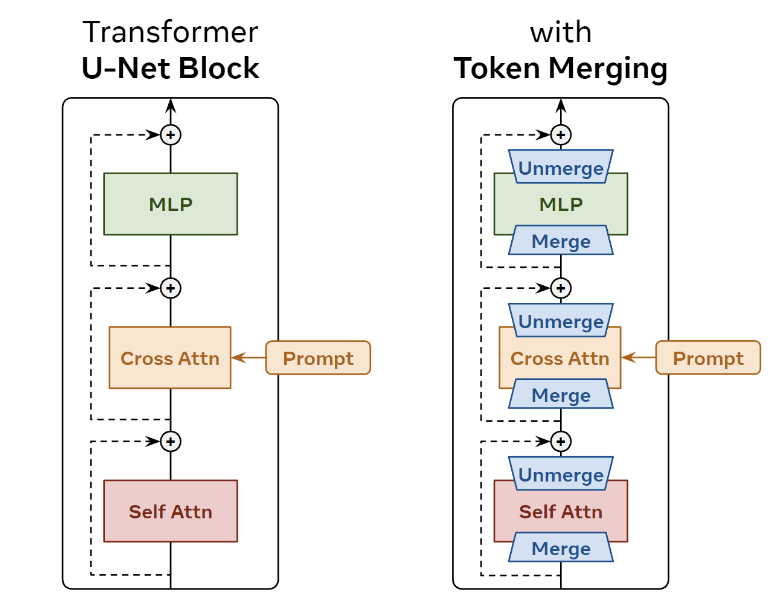
\includegraphics[width=0.55\textwidth]
{static/transformer_graphic.png}
\caption{Transformer with ToMe \cite[Fig.~2]{bolya2023tomesd}.}
\label{fig:tome}
\end{figure}



\subsection{Merge and Unmerge Algorithms}
\subsubsection*{Merging.} The Merge algorithm uses Bipartite-Soft-Matching to determine the similarity of tokens between the \textbf{src} and \textbf{dst} set. The two most similar tokens are repeatedly merged into a new token until the overall number of tokens has reduced by \(r\%\).
Two tokens \(x_1, x_2 \in \mathbb{R}^c\) would be merged into a new token \(x_{1,2}^* \in \mathbb{R}^c \), by averaging their features: \[x_{1,2}^* = \frac{x_1 + x_2}{2}\]



\subsubsection*{Unmerging.} The Unmerge algorithm takes an originally merged token $x_{1,2}^* \in \mathbb{R}^c$ and splits it up into its original tokens $x_1', x_2' \in \mathbb{R}^c$: 
\begin{align*}
    x_1' = x_{1,2}^* \quad\quad
    x_2' = x_{1,2}^*
\end{align*}
in order to recreate the pre-merge amount of tokens.
This naive approach does lose information, as the now unmerged tokens both have the average of their previous values. This loss though is often small (especially for smaller values of \(r\)), as token selection is based on similarity.



\subsection{Bipartite-Soft-Matching}
Bipartite-Soft-Matching involves two main steps. First, the tokens are split into two sets, holding the \textbf{src} and \textbf{dst} tokens respectively. Then, every token in the \textbf{src} set is matched with its most similar token in the \textbf{dst} set, creating a bipartite graph with edges between every \textbf{src} token and their closest match in the \textbf{dst} set. 



\subsubsection*{Choosing src and dst}
The grid of tokens is partitioned into a grid of \(sx \times sy\) batches of tokens.
Within every batch one token is chosen for the \textbf{dst} set (blue) with the rest now belonging to the \textbf{src} set (red). The choice is random by default, alternatively the top left token is always chosen when the parameter \textbf{use\_rand=False} is set (see Fig.~\ref{fig:src-dst}).
\begin{figure}[!htb]
\centering
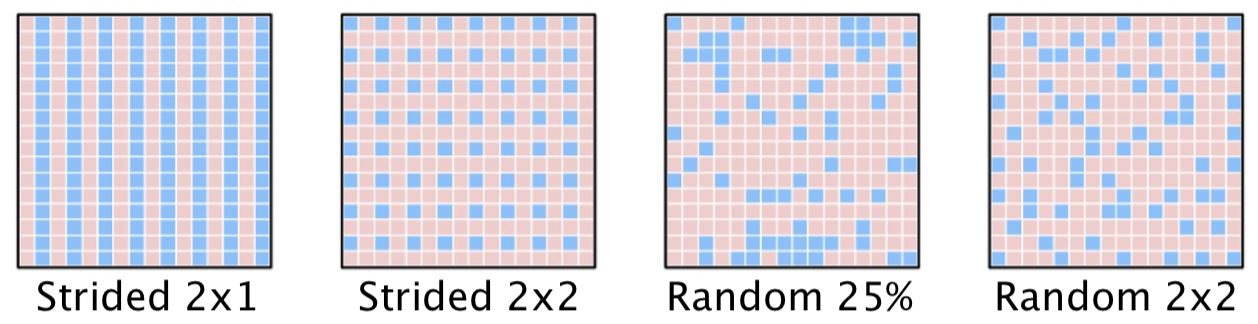
\includegraphics[width=0.75\textwidth]
{static/src_dst_part.png}
\caption{Partitioning of tokens into \textbf{src} and \textbf{dst} \cite[Fig. 5]{bolya2023tome}}
\label{fig:src-dst}
\end{figure}\\
The number of mergeable tokens, which corresponds to the size of the \textbf{src} set, is limited by the choice of \(sx\) and \(sy\).
\begin{align*}
    r_{max} = 1-\frac{1}{sx*sy}
\end{align*}
That means for \(sx = 2\) and \(sy = 2\), no more than 75\% of tokens can be merged.\\
In the subsequent steps, the two most similar tokens are chosen greedily and merged into one, until \(r\%\) of tokens are gone.



\subsection{Token Similarity}
It is also important to define what "token similarity" means in this context. Unlike the first iteration of ToMe which used key-based similarity \cite{bolya2023tome}, ToMe for SD simply partitions the inputs of block \(x\) into to \textbf{src} and \textbf{dst} and then computes the cosine similarity between the two sets. The similarities are only computed once at the beginning of each transformer block \cite{bolya2023tomesd}.



%\newpage
\subsubsection*{Computing cosine similarity}
The token tensor (\(M\)) is normalized and then \(split\) into two tensors (\(S\) and \(D\)), separating the \textbf{src} and \textbf{dst} tokens.
Continuing from there, the cosine similarity (\(scores\)) between every \textbf{src} and \textbf{dst} token is computed by taking the dot product of \(S\) and \(D\).
\begin{lstlisting}[language=Python]
M = M / M.norm(dim=-1, keepdim=True)
S, D = split(M)
scores = S @ D.transpose(-1, -2)
\end{lstlisting}
The \(r\) most similar tokens of \textbf{src} and \textbf{dst} can now be identified by the indices of the largest values of the \(scores\) tensor.



\subsection{Additional Technical Information}
ToMe, in its basic form, only merges tokens in the self-attn layer and defaults to using \(2 \times 2\) batches for token partitioning, with a randomly chosen \textbf{dst} token for every batch, resulting in a 75\% \textbf{src} and 25\% \textbf{dst} split. \\
ToMe is also not applied in every U-Net block, but only the ones with the most tokens. Bolya and Hoffman argued:
"We try restricting ToMe to only blocks with some minimum number of tokens and find that only the blocks with the most tokens need ToMe applied to get most of the speed-up" \cite{bolya2023tomesd}.\\
Lastly, \(r\) remains consistent throughout the whole image generation process, as Bolya and Hoffman found that merging more tokens during earlier diffusion steps and fewer during later steps does not provide a significant improvement to performance.



\subsubsection*{Image inconsistencies}
The usage of ToMe curiously prevents exact reproduction of the subsequent experiments, as minor randomness is involved in the image generation, even when \textbf{use\_rand\\=False} is set. We were not able to determine why this randomness occurs. The variances are detectable by FID, but invisible to the human eye.

\begin{table}[!htb]
\centering
\begin{tabular}{c c c}
    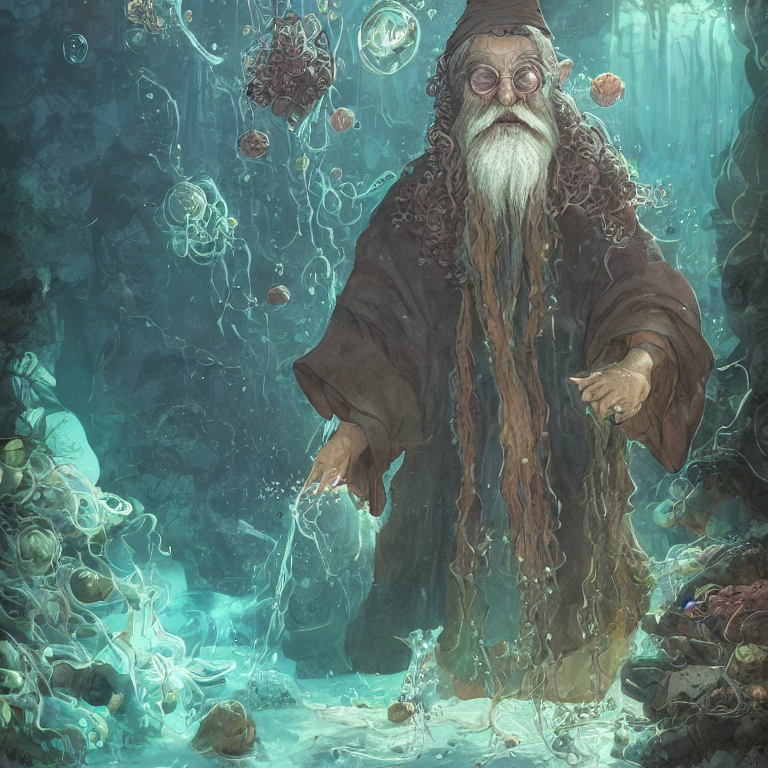
\includegraphics[width=0.3\linewidth]{static/sample_imgs/secondary/wizard_0.png} & 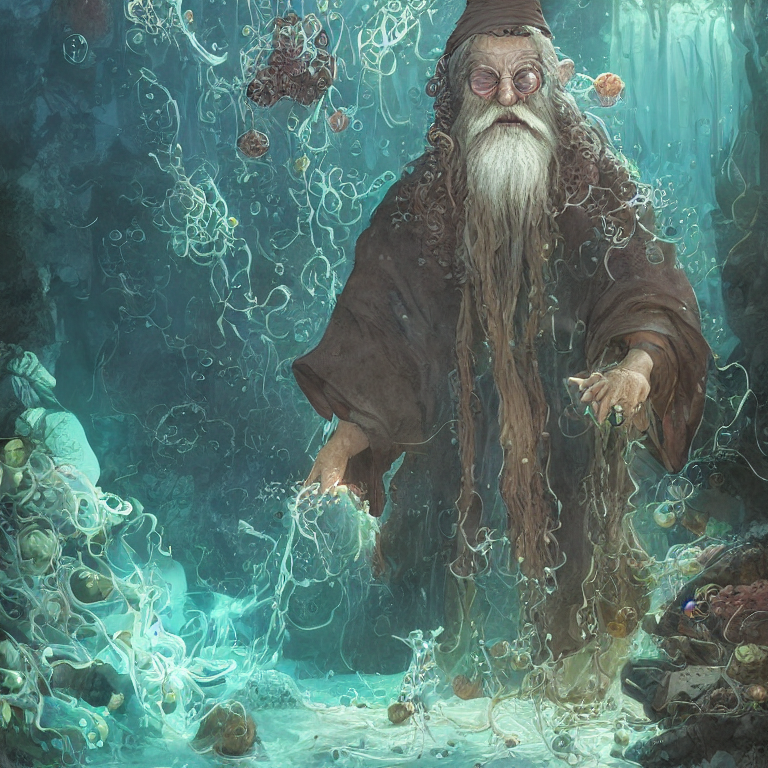
\includegraphics[width=0.3\linewidth]{static/sample_imgs/secondary/wizard_20.png} &
    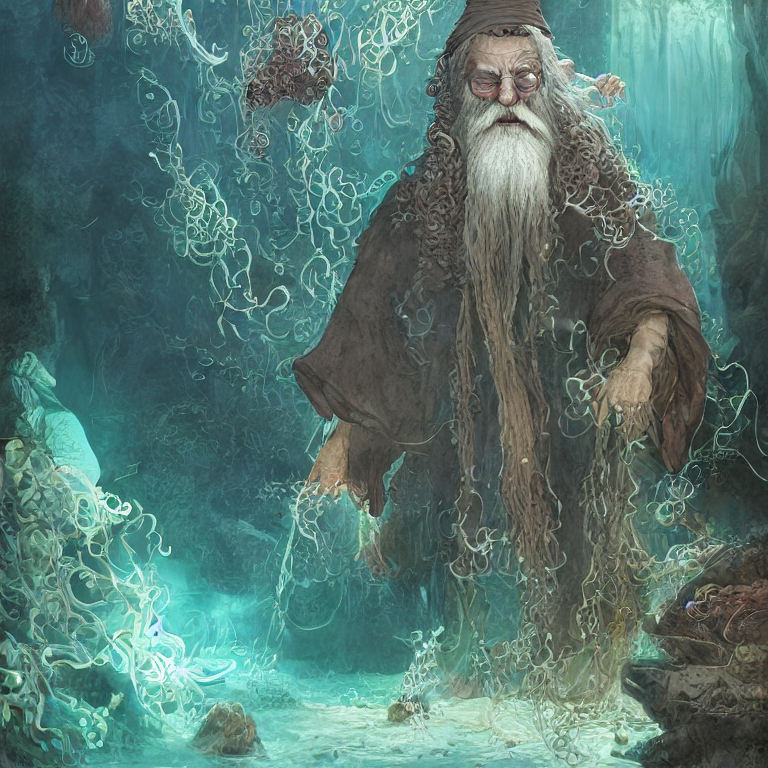
\includegraphics[width=0.3\linewidth]{static/sample_imgs/secondary/wizard_50.png}\\
    \(r=0\%\) & \(20\%\) & \(50\%\) \\
\end{tabular}
\caption{$768 \times 768$ images created with the default configuration of ToMe}
\end{table}
